%%%%%%%%%%%%%%%%%%%%%%%%%%%%%%%%%%%%%%%%%
% University Assignment Title Page 
% LaTeX Template
% Version 1.0 (27/12/12)
%
% This template has been downloaded from:
% http://www.LaTeXTemplates.com
%
% Original author:
% WikiBooks (http://en.wikibooks.org/wiki/LaTeX/Title_Creation)
%
% License:
% CC BY-NC-SA 3.0 (http://creativecommons.org/licenses/by-nc-sa/3.0/)
% 
% Instructions for using this template:
% This title page is capable of being compiled as is. This is not useful for 
% including it in another document. To do this, you have two options: 
%
% 1) Copy/paste everything between \begin{document} and \end{document} 
% starting at \begin{titlepage} and paste this into another LaTeX file where you 
% want your title page.
% OR
% 2) Remove everything outside the \begin{titlepage} and \end{titlepage} and 
% move this file to the same directory as the LaTeX file you wish to add it to. 
% Then add \input{./title_page_1.tex} to your LaTeX file where you want your
% title page.
%
%%%%%%%%%%%%%%%%%%%%%%%%%%%%%%%%%%%%%%%%%

%----------------------------------------------------------------------------------------
%	PACKAGES AND OTHER DOCUMENT CONFIGURATIONS
%----------------------------------------------------------------------------------------

\documentclass[12pt]{article}
\usepackage[utf8]{inputenc}
\usepackage[russian]{babel}
\usepackage{amsmath,amsfonts,amsthm} % Math packages
\usepackage{mathtools}
\usepackage{graphicx}
\usepackage{booktabs}
\usepackage[margin=1.15in]{geometry}
\usepackage{accents}
\usepackage{url}
\usepackage{caption}
\usepackage{subcaption}
\usepackage{textcomp}
\DeclareGraphicsExtensions{.pdf,.png,.jpg}

\usepackage{lipsum} % Used for inserting dummy 'Lorem ipsum' text into the template

\usepackage{sectsty} % Allows customizing section commands
\allsectionsfont{\centering \normalfont\scshape} % Make all sections centered, the default font and small caps

\usepackage{fancyhdr} % Custom headers and footers
\pagestyle{fancyplain} % Makes all pages in the document conform to the custom headers and footers
\fancyhead{} % No page header - if you want one, create it in the same way as the footers below
\fancyfoot[L]{} % Empty left footer
\fancyfoot[C]{} % Empty center footer
\fancyfoot[R]{\thepage} % Page numbering for right footer
\renewcommand{\headrulewidth}{0pt} % Remove header underlines
\renewcommand{\footrulewidth}{0pt} % Remove footer underlines
\setlength{\headheight}{13.6pt} % Customize the height of the header

\numberwithin{equation}{section} % Number equations within sections (i.e. 1.1, 1.2, 2.1, 2.2 instead of 1, 2, 3, 4)
\numberwithin{figure}{section} % Number figures within sections (i.e. 1.1, 1.2, 2.1, 2.2 instead of 1, 2, 3, 4)
\numberwithin{table}{section} % Number tables within sections (i.e. 1.1, 1.2, 2.1, 2.2 instead of 1, 2, 3, 4)

\setlength\parindent{0pt} % Removes all indentation from paragraphs - comment this line for an assignment with lots of text

\begin{document}

\begin{titlepage}

\newcommand{\HRule}{\rule{\linewidth}{0.5mm}} % Defines a new command for the horizontal lines, change thickness here

\center % Center everything on the page
 
%----------------------------------------------------------------------------------------
%	HEADING SECTIONS
%----------------------------------------------------------------------------------------

\textsc{\Large київський національний університет імені тараса шевченка}\\[1.5cm] % Name of your university/college
\textsc{\large факультет комп'ютерних наук та кібернетики}\\[0.5cm] % Major heading such as course name
\textsc{\large кафедра прикладної математики}\\[0.5cm] % Minor heading such as course title

%----------------------------------------------------------------------------------------
%	TITLE SECTION
%----------------------------------------------------------------------------------------

\HRule \\[0.4cm]
{ \Large \bfseries Лабораторна робота №3 з курсу “Чисельні методи математичної фізики”:}\\[0.4cm] % Title of your document
{ \Large \bfseries “Розв'язання задачі теплопровідності” }
\HRule \\[1.5cm]
 
%----------------------------------------------------------------------------------------
%	AUTHOR SECTION
%----------------------------------------------------------------------------------------

\begin{minipage}{0.4\textwidth}
\begin{flushleft} \large
\emph{Студент 4-го курсу}\\
\emph{групи ОМ}\\
Чан Ха Ву % Your name
\end{flushleft}
\end{minipage}
~
\begin{minipage}{0.4\textwidth}
\begin{flushright} \large
\emph{Викладач:} \\
\emph{к.ф.-м.н., доцент} \\
Риженко \textsc{А. І.} % Supervisor's Name
\end{flushright}
\end{minipage}\\[4cm]

% If you don't want a supervisor, uncomment the two lines below and remove the section above
%\Large \emph{Author:}\\
%John \textsc{Smith}\\[3cm] % Your name

%----------------------------------------------------------------------------------------
%	DATE SECTION
%----------------------------------------------------------------------------------------

{\large Київ, 01 січня 2017}\\[3cm] % Date, change the \today to a set date if you want to be precise

%----------------------------------------------------------------------------------------
%	LOGO SECTION
%----------------------------------------------------------------------------------------

%\includegraphics{Logo}\\[1cm] % Include a department/university logo - this will require the graphicx package
 
%----------------------------------------------------------------------------------------

\vfill % Fill the rest of the page with whitespace
\end{titlepage}

\renewcommand{\refname}{Літератури та посилання}
\renewcommand{\figurename}{Мал.}

%----------------------------------------------------------------------------------------
%	ПОСТАНОВКА ЗАДАЧИ
%----------------------------------------------------------------------------------------
\section{Постановка задачі}

Цегло сферичної форми діаметром \( 2R = 20\text{мм}\), що має початкову температуру \(0 {^\circ}C\), вміщено в піч, температура якої дорівнює \(300 {^\circ}C\). Визначити, через який час температура в середині цієї цеглини дорівнюватиме \(30 {^\circ}C\). Фізичні характеристики цегла мають такі значення:

\begin{equation}
\begin{multlined} \label{text:data}
\lambda = 0,77 \,\frac{\text{Вт}}{\text{м}\cdot\text{К}}; \quad c = 0,83 \,\frac{\text{кДж}}{\text{кг}\cdot\text{К}}; \quad \rho = 1600 \,\frac{\text{кг}}{\text{м}^3}; \quad \gamma = 7 \,\frac{\text{Вт}}{\text{м}^2 \cdot \text{К}}.
\end{multlined}
\end{equation}

Тут \(c\) -- питомна щільність, \(\rho\) -- щільність, \(\lambda\) -- коефіцієнт теплопровідності, \(\gamma\) -- коефіцієнт тепловіддачі на границі.

%----------------------------------------------------------------------------------------
%	РЕШЕНИЕ
%----------------------------------------------------------------------------------------
\section{Хід розв'язку}

Процес нагрівання ідеально сферичної цеглини може бути описаний таким диференціальним рівнянням:

\begin{equation}
\begin{multlined} \label{init:problem}
c\rho\frac{\partial u}{\partial t} = \frac{\lambda}{x^2}\frac{\partial}{\partial{x}}\left(x^2\frac{\partial{u}}{\partial{x}}\right), \quad x \in (0, R), \quad t > 0
\end{multlined}
\end{equation}

Початкові та крайові умови при параметрах (\ref{text:data}) запишемо у такому вигляді:

\begin{equation}
\begin{split} \label{init:conditions}
\left.u(x, t)\right|_{t = 0} = 0 \quad \forall x \in [0, R]; \quad \left.x^2\frac{\partial{u}}{\partial{x}}\right|_{x \rightarrow 0} = 0\\ 
\left.\left(\lambda\frac{\partial{u}}{\partial{x}} + \gamma(u - u_\text{env})\right)\right|_{x=R} = 0, \quad \forall t > 0.
\end{split}
\end{equation}

де \( R = 10^{-2}\text{м}\), \(u_\text{env} = 300{^\circ}C\).

\subsection{Зведення до безрозмірного випадку}
Перетворимо задачу (\ref{init:problem}), (\ref{init:conditions}) таким чином, щоб пропали коефіцієнти теплопровідності, щільності, питомної щільності та тепловіддачі. Введемо безрозмірні змінні

\begin{equation}
\begin{split} \label{sol:newsys}
v(x, t) = \frac{(u(x, t) - u_\text{cont})}{u_\text{cont}}; \quad \hat{t} = \frac{a^2t}{R^2}, \quad \hat{x} = x/R;
\end{split}
\end{equation}

де \( a^2 = \lambda/(c\rho)\); \(u_\text{cont}\) -- деяка величина, яка відповідає, наприклад, \( u_{\text{env}}\). Переходячі в задачі (\ref{init:problem}), (\ref{init:conditions}) до безрозмірних змінних за формулами (\ref{sol:newsys}), дістаємо таку задачу для функції \( v\left(\hat{x}, \hat{t}\right)\):

\begin{equation}
\begin{split} \label{nomes:problem}
\frac{\partial{v}}{\partial{\hat{t}}} = \frac{1}{\hat{x}^2} \, \frac{\partial}{\partial \hat{x}} \left( \hat{x}^2 \, \frac{\partial v}{\partial \hat{x}} \right), \quad \hat{x} \in (0, 1), \quad t > 0
\end{split}
\end{equation}

при чому початкові та крайові умови набудуть наступний вигляд:

\begin{equation}
\begin{multlined} \label{nomes:conditions}
\left.v(\hat{x}, \hat{t})\right|_{t = 0} = v_0(\hat{x}) \quad \forall \hat{x} \in [0, 1];\\ \\
\left.\left( \frac{\partial v}{\partial \hat{x}} + \hat{\gamma}v\right)\right|_{\hat{x} = 1} = 0, \quad \left.\hat{x}^2\frac{\partial{v}}{\partial{\hat{x}}}\right|_{\hat{x} \rightarrow 0} = 0.
\end{multlined}
\end{equation}

де \( v_0(\hat{x}) = (u_0(x) - u_\text{cont})/u_\text{cont}\); \(\hat{\gamma} = \gamma R\lambda\).

\subsection{Апроксимізація різницевою схемою}

Введемо сітку \( \overline{\omega}_{h,t} = \overline{\omega}_h \times \overline{\omega}_t\), де \( \overline{\omega}_h = \left\{ x_i = ih, h = \frac{1}{N}, i = 0, 1, \dots N\right\}\). При чому для кожного фіксованого \( \tau\), \( \overline{\omega}_t = \left\{t_j = j\tau, j = 0, 1, \dots M\right\}\). 
\bigskip

Надалі для зручності будемо вважати, що наше рівняння має вигляд (змінені лише назви змінних):

\begin{equation}
\begin{multlined} \label{simplified}
\frac{\partial U}{\partial t} = \frac{1}{x^2} \frac{\partial}{\partial x} \left( x^2 \frac{\partial U}{\partial x}\right)
\end{multlined}
\end{equation}

Введемо заміну

\begin{equation}
\begin{multlined} \label{simplified}
W = x \frac{\partial U}{\partial x}
\end{multlined}
\end{equation}

Далі помножимо обидві частини на \( x\), і проінтегруємо наше початкове рівняння на проміжку \(x \in [x_{i-\frac{1}{2}}, x_{i+\frac{1}{2}}]\) і поділимо обидві частини на \( h\):

\begin{equation}
\begin{multlined} \label{simplified}
\frac{1}{h} \int_{x_{i - \frac{1}{2}}}^{x_{i+\frac{1}{2}}} {x\frac{\partial U}{\partial t}}\,dx = \frac{1}{h} \int_{x_{i - \frac{1}{2}}}^{x_{i+\frac{1}{2}}} {\frac{\partial W}{\partial x}}\,dx
\end{multlined}
\end{equation}

Використовуючи теорему про середнє значення, винесемо \( \frac{\partial U}{\partial t}\) за межі першої частини інтегралу і праву частину, враховуючи \( w_i = w(x_i)\). Отримаємо

\begin{equation}
\begin{multlined} \label{simplified}
\frac{\partial U_i}{\partial t} \times \frac{1}{h} \int_{x_{i-\frac{1}{2}}}^{x_{i-\frac{1}{2}}} {x}\,dx = \frac{1}{h}\left( w_{i + \frac{1}{2}} - w_{i - \frac{1}{2}}\right)
\end{multlined}
\end{equation}


Як показано у \cite[с. 185-208]{Samarskii71}, безрозмірна задача теплопровідності у сферичних координатах (\ref{nomes:problem}), (\ref{nomes:conditions}) за допомогою інтегро-інтерполяційного метода можна апроксимувати такою системою:

\begin{equation}
\begin{multlined} \label{nomes:approx}
\Lambda(\overline{t}) y = \frac{1}{x^2}\left(x^2 y_{\,\overline{x}}\right)_x, \quad \overline{x} = x - \frac{h}{2}, \quad \overline{t} = t + \frac{h}{2}
\end{multlined}
\end{equation}

Отже, рівняння та крайові умови можна записати таким чином:

\begin{align}
\left\{\begin{array}{c}
y_t = \Lambda(\overline{t})y, \quad 0 < x = ih < 1, \quad t = j\tau > 0\\
y(x, 0) = u_0(x), \quad y(1, t) = u_\text{cont}\\
y^{(\sigma)} = \sigma\hat{y} + (1 - \sigma)y
\end{array}\right.
\end{align}

Маємо:

\begin{align} \label{diff:approx}
\left\{\begin{array}{c}
y_{t, i}^j = \sigma \frac{1}{x_i^2}\left( x_{i-\frac{1}{2}}^2 y_{\overline{x}}^{j+1}\right)_{x, i} + (1-\sigma)\left( x_{i-\frac{1}{2}}^2 y_{\overline{x}}^j\right) \\ \\
\sigma y_{x, 0}^{j+1} + (1-\sigma)y_{x, 0}^j = \frac{h}{2 \cdot 3} y_{t, 0}^j \\\\
-\sigma y_{x, N}^{j+1} - (1 -\sigma)y_{x, N}^j = \hat{\gamma} \left( \sigma y_{N}^{j+1} + (1-\sigma)y_N^j\right) + \frac{h}{2}y_{t, N}^j
\end{array}\right. 
\end{align}

Побудуємо тридіагональну систему рівнянь для \( j+1\) шару

\begin{align} \label{diff:approx}
\left\{\begin{array}{c}
d_0y_0^{j+1} + c_0y_1^{j+1} = f_0\\\\
l_iy_{i-1}^{j+1} + d_iy_i^{j+1} + u_iy_{i+1}^{j+1} = f_i\\\\
l_Ny_{N-1}^{j+1} + d_Ny_N^{j+1} = f_N
\end{array}\right. 
\end{align}

де коефіцієнти обчислюється наступним чином:

\begin{align} \label{diff:tridiag}
\begin{split}
d_0 = \frac{-\sigma}{h} - \frac{h}{2 \cdot 3\tau}, \quad u_0 = \frac{\sigma}{h}, \quad f_0 = -(1-\sigma)\frac{y_1^j - y_0^j}{h} - \frac{h}{2 \cdot 3} \frac{y_0^j}{\tau} \\
l_i = \frac{-\sigma x_{i-\frac{1}{2}}^2}{h^2 x_i^2}, \quad d_i = \frac{1}{\tau} + \frac{\sigma \left( x_{i-\frac{1}{2}}^2 +x_{i+\frac{1}{2}}^2 \right)}{h^2 x_i^2}, \quad u_i = \frac{-\sigma x_{i+\frac{1}{2}}^2}{h^2 x_i^2}\\
f_i =\frac{y_i^j}{\tau} + (1-\sigma)\frac{1}{x_i^2} \left( \frac{x_{i+\frac{1}{2}}^2 y_{i+1}^j - \left( x_{i-\frac{1}{2}}^2 + x_{1+\frac{1}{2}}^2 \right)y_i^j + x_{i-\frac{1}{2}}^2 y_{i-1}^j }{h^2}\right)\\
l_N = -\frac{\sigma}{h}, \quad d_N = \frac{\sigma}{h} + \hat{\gamma}\sigma + \frac{h}{2\tau}\\f_N = -(1-\sigma)\left( \frac{y_N^j - y_{N-1}^j}{h} + \hat{\gamma}y_N^j\right) + \frac{h}{2\tau}y_N^j
\end{split}
\end{align}

Для нульового шару при \(j = 0\) розв'язок задачі теплопровідності збігається з початковими умовами.

%----------------------------------------------------------------------------------------
%	ПРАКТИЧНА ЧАСТИНА
%----------------------------------------------------------------------------------------

\section{Практична частина}

Для розв'язання тридіагональної системи (\ref{diff:tridiag}) будемо використовувати метод прогонки, який працює за \(O(n)\), де \( n \) -- розмір матриці. Розв'язок системи щукається у вигляді

\begin{equation}
\begin{multlined} \label{diff:solve_tridiag}
y_i = s_i + y_{i+1} + t_i, \quad i = 0, 1, \dots n-1.
\end{multlined}
\end{equation}

Коефіцієнти \(s_i\) та \(t_i\) щукається наступним чином. З системи (\ref{diff:tridiag}) можна побачити, що

\begin{equation}
\begin{multlined} 
s_0 = \frac{C_0}{B_0}, \quad t_0 = \frac{-G_0}{B_0}.
\end{multlined}
\end{equation}

Підставимо \( y_{i-1} \) у \(i\)-му рівнянні системи:

\begin{equation}
\begin{multlined} 
A_i\left(s_{i-1}y_i + t_{i-1}\right) - B_i y_i + C_iy_{i+1} = G_i,
\end{multlined}
\end{equation}

отримаємо рекурентну формулу:

\begin{equation}
\begin{multlined} 
s_i = \frac{C_i}{B_i-A_is_{i-1}}, \quad t_i = \frac{A_it_{i-1}-G_i}{B_i-A_is_{i-1}}, \quad i = 1, 2, \dots n.
\end{multlined}
\end{equation}

У \(n\)-му рівнянні системи (\ref{diff:tridiag}) \(C_n = 0\), отже, \(s_n = 0\), значить з (\ref{diff:solve_tridiag}) випливає що \(y_n = t_n\). По формулі (\ref{diff:solve_tridiag}) знаходимо остальні коефіцієнти.

%----------------------------------------------------------------------------------------
%	РЕЗУЛЬТАТ РОБОТИ
%----------------------------------------------------------------------------------------

\section{Результат роботи програми}
\begin{figure}[h!]
  \centering
  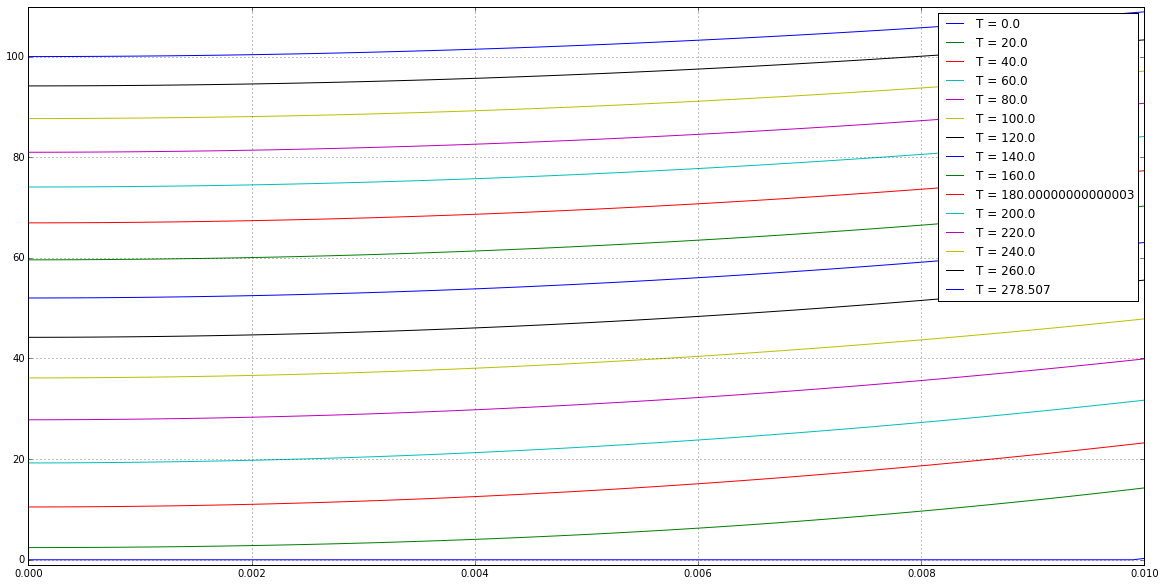
\includegraphics[width=.9\linewidth]{res0}
  \caption{\it \( u(t)\) при фіксованому \(t\).}
\end{figure}

\begin{figure}[h!]
  \centering
  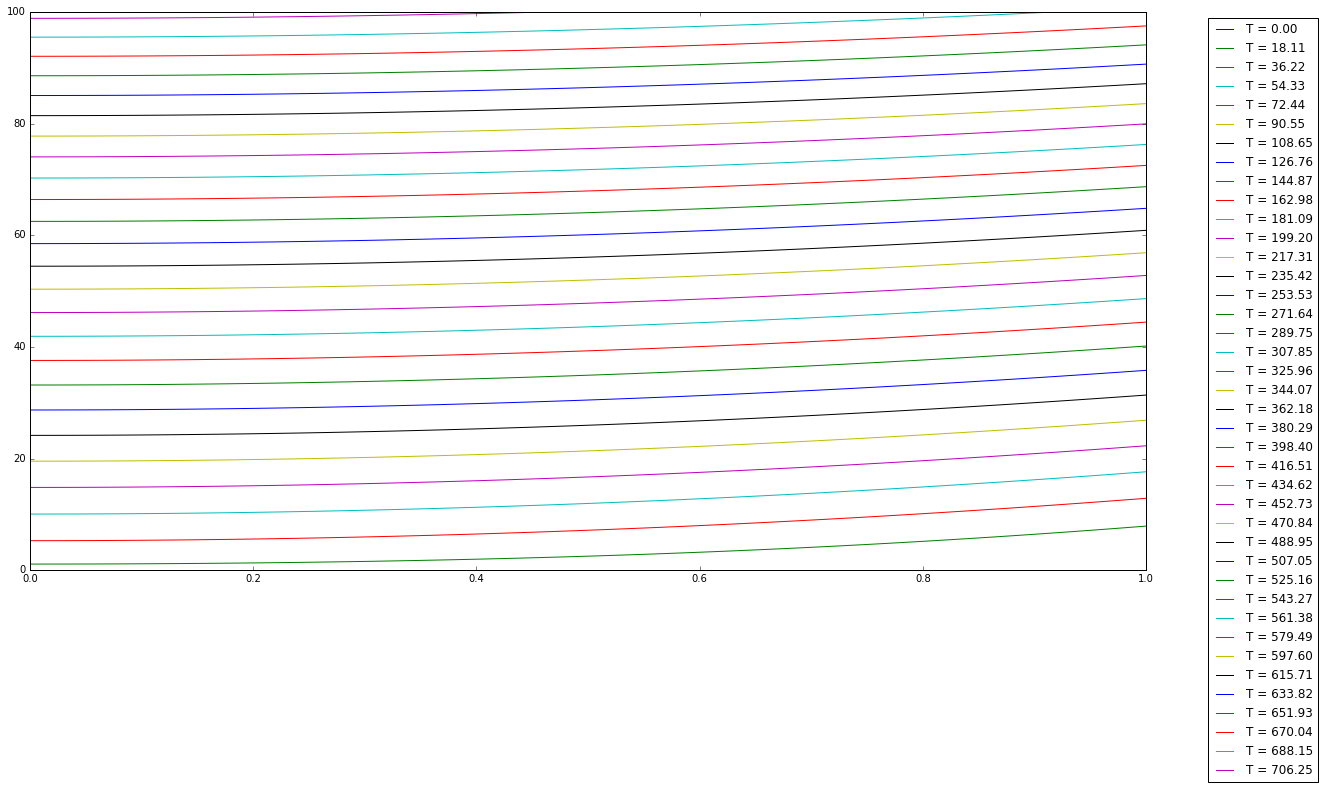
\includegraphics[width=.9\linewidth]{res1}
  \caption{\it \( u(t)\) при фіксованому \(t\).}
\end{figure}

\begin{thebibliography}{9}

\bibitem{Samarskii71}
  А. А. Самарский,
  \emph{Введение в теорию разностных схем},
  Главная редакция физико-математической литературы изд-ва «Наука», 
  М., 1971. 
\bibitem{SourceCode}
  Чан Х. В., \emph{Метод безпосередньої заміни диференціальних похідних частковими на мові Python 3}, 2017. 
  \url{https://github.com/FalconUA/numerical-analysis/blob/master/s3-3/appointment_s3-3.ipynb}

\end{thebibliography}
\end{document}